\documentclass[twocolumn]{IEEEtran}
\usepackage{graphicx}
\usepackage[utf8x]{inputenc}
\usepackage{times}
\usepackage{amssymb,amsfonts}
\usepackage{pict2e}
\usepackage{float}
\usepackage[all]{xy}
\usepackage{graphics,graphicx,color,colortbl}
\usepackage{subfigure}
\usepackage{wrapfig}
\usepackage{multicol}
\usepackage{cite}
\usepackage{url}
\usepackage[tbtags]{amsmath}
\usepackage{amsmath,amssymb,amsfonts,amsbsy}
\usepackage{bm}
\usepackage{listings}
\usepackage{algorithm}
\usepackage{algorithmic}
\usepackage[centerlast, small]{caption}
\usepackage[colorlinks=true, citecolor=blue, linkcolor=blue, urlcolor=blue, breaklinks=true]{hyperref}
\hyphenation{ele-men-tos he-rra-mi-en-ta cons-tru-yen trans-fe-ren-ci-a pro-pu-es-tas si-mu-lar re-que-ri-mien-tos}

\begin{document}
\title{Control PID}
\author{Israel Ricardo Bernal Sánchez Código: $261613$\\
	Felipe Castañeda Prieto Código $285728$\\
	David Ricardo Martínez Hernández Código: $261931$\\
	Oscar Andrés Urbano Vallejo Código: $261683$}
\maketitle
\markboth{Universidad Nacional de Colombia}{}
\floatname{algorithm}{Algoritmo}

\begin{abstract}

\end{abstract}
\begin{keywords}
 
\end{keywords}

\section{Introducción}
\noindent


\section{Procedimiento}
\noindent
\subsection{Modelado y Validación}
\noindent
\begin{figure}[H]
	\centering
		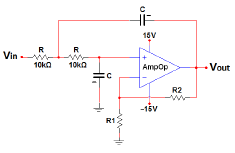
\includegraphics[scale=1.2]{montaje1.png}
	\caption{Circuito de la planta a controlar.}
	\label{fig1}
\end{figure}

\subsection{Diseño de los compensadores}

\subsubsection{Punto 4.2.1 y 4.2.3}

\subsubsection{Punto 4.2.4}

\subsubsection{Punto 4.2.5}
\noindent
Para diseñar el compensador de adelanto de fase para la Fig \ref{fig1}, tal que alcance los siguientes requerimientos:
%cll 16 n 16-80, clinica candelaria sede centro dual, 1 cuadra arriba estacion sabana, frente a una iglesia
\begin{itemize}
 \item Error de posición inferior a $3 \%$.
 \item Margen de fase $\geq 55°$.
 \item Margen de ganancia $\geq 10dB$.
\end{itemize}
\noindent
se utilizó el siguiente procedimiento:
\begin{enumerate}
 \item Se calculo la constante del error de posición para el error permanente y se determino la ganancia $K_c$ que cumple ese criterio:
\begin{equation}
 e_{ss_{p}}=\frac{200K_c}{100+200K_c} \leq 3\%
\label{ecu1}
\end{equation}
\begin{equation}
 E=R-Y \Longrightarrow Y=\frac{200K_c}{100+200K_c} R
\label{ecu2}
\end{equation}
\begin{equation}
 E=R-\frac{200K_c}{100+200K_c} R;\ \ R=1
\label{ecu3}
\end{equation}
\begin{equation}
 E=1-\frac{200K_c}{100+200K_c}
\label{ecu4}
\end{equation}
\begin{equation}
3 \% \leq 1-\frac{200K_c}{100+200K_c};\ \ K_c < -\frac{1}{2}\ \ y \ \ K_c \geq \frac{97}{6}
\label{ecu5}
\end{equation}
 \item Se determino la frecuencia de cruce de ganancia $\omega _g$
\begin{equation}
 \omega _g \Longrightarrow \left| {G\left( s \right)_{\left| {_{s = i\omega } } \right.} } \right| = 1
\label{ecu6}
\end{equation}
\begin{equation}
 \omega _g = 56.9254483053852;\ \ \omega _p=\infty;\ \ 
\label{ecu}
\end{equation}
\begin{equation}
 
\label{ecu}
\end{equation}
\begin{equation}
 
\label{ecu}
\end{equation}
\begin{equation}
 
\label{ecu}
\end{equation}
\begin{equation}
 
\label{ecu}
\end{equation}
 \item 

\item 
\end{enumerate}


\section{Conclusiones}
\noindent
\begin{itemize}
 \item 
 \item 
 \item 
 \item 
\end{itemize}


\bibliographystyle{ieeetran}
\begin{thebibliography}{99}

\bibitem{chen} Chen, Chi-Tsong.
{\em "`Analog and Digital Control System Desing: Transfer-Function, State, Space and Algebraic Methods"'}.
Saunders College Publishing, 1993.

\bibitem{kuo} Kuo, C. Benjamin.
{\em "`Sistemas Automáticos de Control"'}.
Pentice Hall Hispanoamerica, Séptima Edición, 1996.

\bibitem{ogata} Ogata, Katsuhiko.
{\em "`Ingeniería De Control Moderna"'}.
Pearson Educación, Tercera Edición, 1998.

\end{thebibliography}
\end{document}